\documentclass[10pt,a4paper]{article}
\usepackage[utf8]{inputenc}
\usepackage{amsmath,amssymb}
\usepackage{graphicx}
\usepackage{booktabs}
\usepackage{array}
\usepackage[margin=0.75in]{geometry}
\usepackage{caption}
\usepackage{microtype}
\usepackage{titlesec}
\usepackage{float}
\usepackage{xcolor}
\usepackage{colortbl}
\usepackage{hyperref}

\definecolor{highlightcol}{RGB}{255,235,180}
\definecolor{navyheader}{RGB}{20,40,80}

\titleformat{\section}{\large\bfseries\color{navyheader}\raggedright}{}{0pt}{}[\vspace{1pt}\hrule height 0.8pt]
\titleformat{\subsection}{\normalfont\bfseries\color{navyheader}\raggedright}{}{0pt}{}

\captionsetup{font=small,labelfont=bf}

\title{\textbf{\Large Evaluación Biomecánica Transmural de la Arteria Carótida Común:}\\[2pt]
\large Formulación Constitutiva, Integración de Pared Gruesa, Modelo Perivascular In Vivo y Comparación Ex Vivo}
\author{\textbf{Simulación Biomecánica y Mecánica de Medios Continuos}}
\date{30 de Septiembre de 2026}

\begin{document}

\maketitle

\begin{abstract}
\noindent Este documento presenta la formulación rigurosa de Mecánica de Medios Continuos para la determinación de la presión intraluminal ($P_i$) en arterias carótidas comunes humanas (CCA), integrando los modelos \textit{in vivo} de Masson et al. (2011) con los ensayos \textit{ex vivo} del complejo Media-Íntima de Sommer \& Holzapfel (2012). Se incorpora el análisis del confinamiento perivascular ($P_a$), la formulación simplificada de Santiago Urquiza (Tesis Doctoral, Cap. 3) evaluada en el radio medio ($r_m$), la demostración analítica del sesgo positivo de la Ley de Laplace mediante series de Taylor, las deducciones analíticas explícitas de $P_i(\lambda_\theta)$, la comparación funcional de la approximante de Padé [1/1] y la función analítica optimizada $P_i(\lambda_\theta) = 0.1427 \cdot (e^{11.9103(\lambda_\theta - 1)} - 1)$ [kPa].
\end{abstract}

\section{1. Figuras Originales de la Literatura Primaria}
\noindent En esta sección se presentan las figuras originales publicadas por sus autores en la literatura científica primaria:

\begin{figure}[H]
\centering
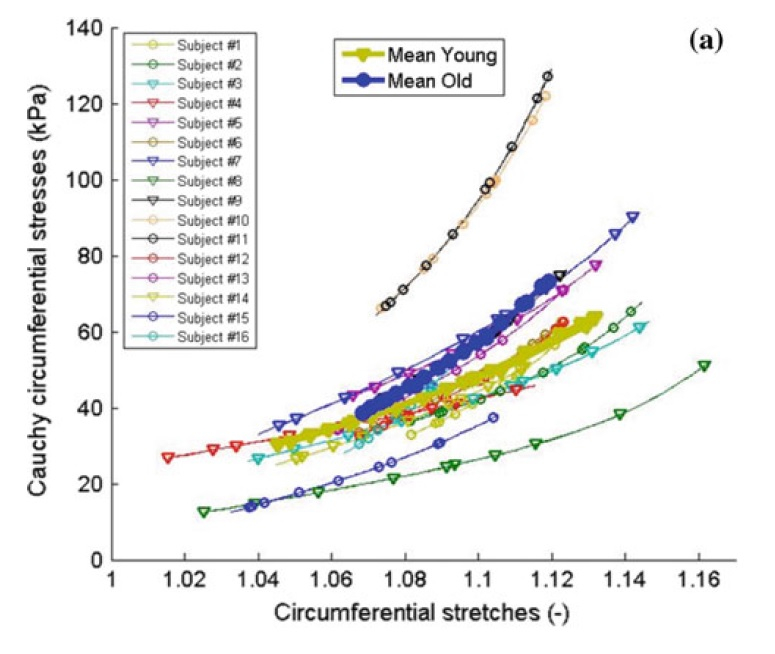
\includegraphics[width=0.62\linewidth]{Figura 5a_Masson.jpg}
\caption{\textbf{Figura 5a Original (Masson et al., 2011)}: Tensión de Cauchy Circunferencial $\sigma_{\theta\theta}$ [kPa] vs. Estiramiento Circunferencial $\lambda_\theta$ para Jóvenes Normotensos (\textit{Mean Young}, 21--42a) y Mayores Normotensos (\textit{Mean Old}, 53--64a).}
\label{fig:orig_5a_masson}
\end{figure}

\begin{figure}[H]
\centering
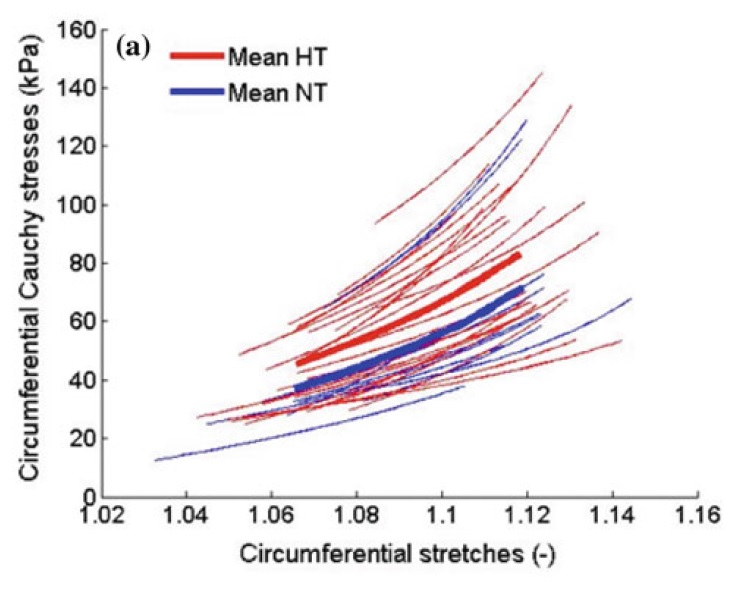
\includegraphics[width=0.62\linewidth]{Figura 7a_Masson.jpg}
\caption{\textbf{Figura 7a Original (Masson et al., 2011)}: Tensión de Cauchy Circunferencial $\sigma_{\theta\theta}$ [kPa] vs. Estiramiento Circunferencial $\lambda_\theta$ para Hipertensos Tratados (\textit{Mean HT}, 44--69a) frente a Normotensos (\textit{Mean NT}).}
\label{fig:orig_7a_masson}
\end{figure}

\begin{figure}[H]
\centering
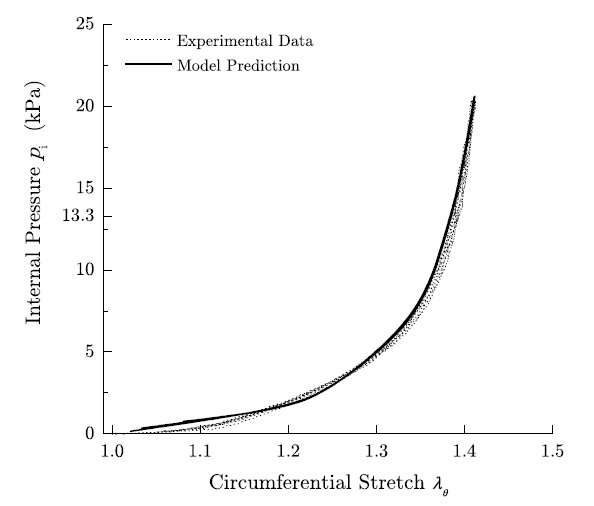
\includegraphics[width=0.62\linewidth]{Figura_6a_Sommer_&_Holzapfel.jpg}
\caption{\textbf{Figura 6a Original (Sommer \& Holzapfel, 2012)}: Presión Intraluminal $P$ [kPa / mmHg] vs. Estiramiento Circunferencial $\lambda_\theta$ para el complejo Media-Íntima de Carótida Común (\textit{Donante VI r}).}
\label{fig:orig_6a_sommer}
\end{figure}

\section{2. Desarrollo Físico, Cinemático y Constitutivo Riguroso}

\subsection{2.1 Método de Medición Indirecta No Invasiva por Ultrasonido (Ecotracking)}
En la caracterización clínica \textit{in vivo} de la carótida común (Masson et al., 2011), la respuesta mecánica se determina de manera no invasiva acoplando ecotracking ultrasónico de alta resolución (diámetro interno $2r_i(t)$ y espesor íntima-media $h(t)$) y tonometría de aplanamiento (presión sanguínea intraluminal $P_i(t)$).

\subsection{2.2 Cinemática y Condición de Incompresibilidad}
Bajo incompresibilidad estricta del tejido vascular ($J = \det \mathbf{F} = 1$):
\begin{equation}
J = \lambda_r \lambda_\theta \lambda_z = 1 \implies \lambda_r = \frac{1}{\lambda_\theta \lambda_z}
\end{equation}

\subsection{2.3 Esquema Transmural de la Arteria}
A continuación se muestra el esquema cilíndrico de la sección transversal arterial que define gráficamente las variables geométricas y mecánicas de las ecuaciones de equilibrio:

\begin{figure}[H]
\centering
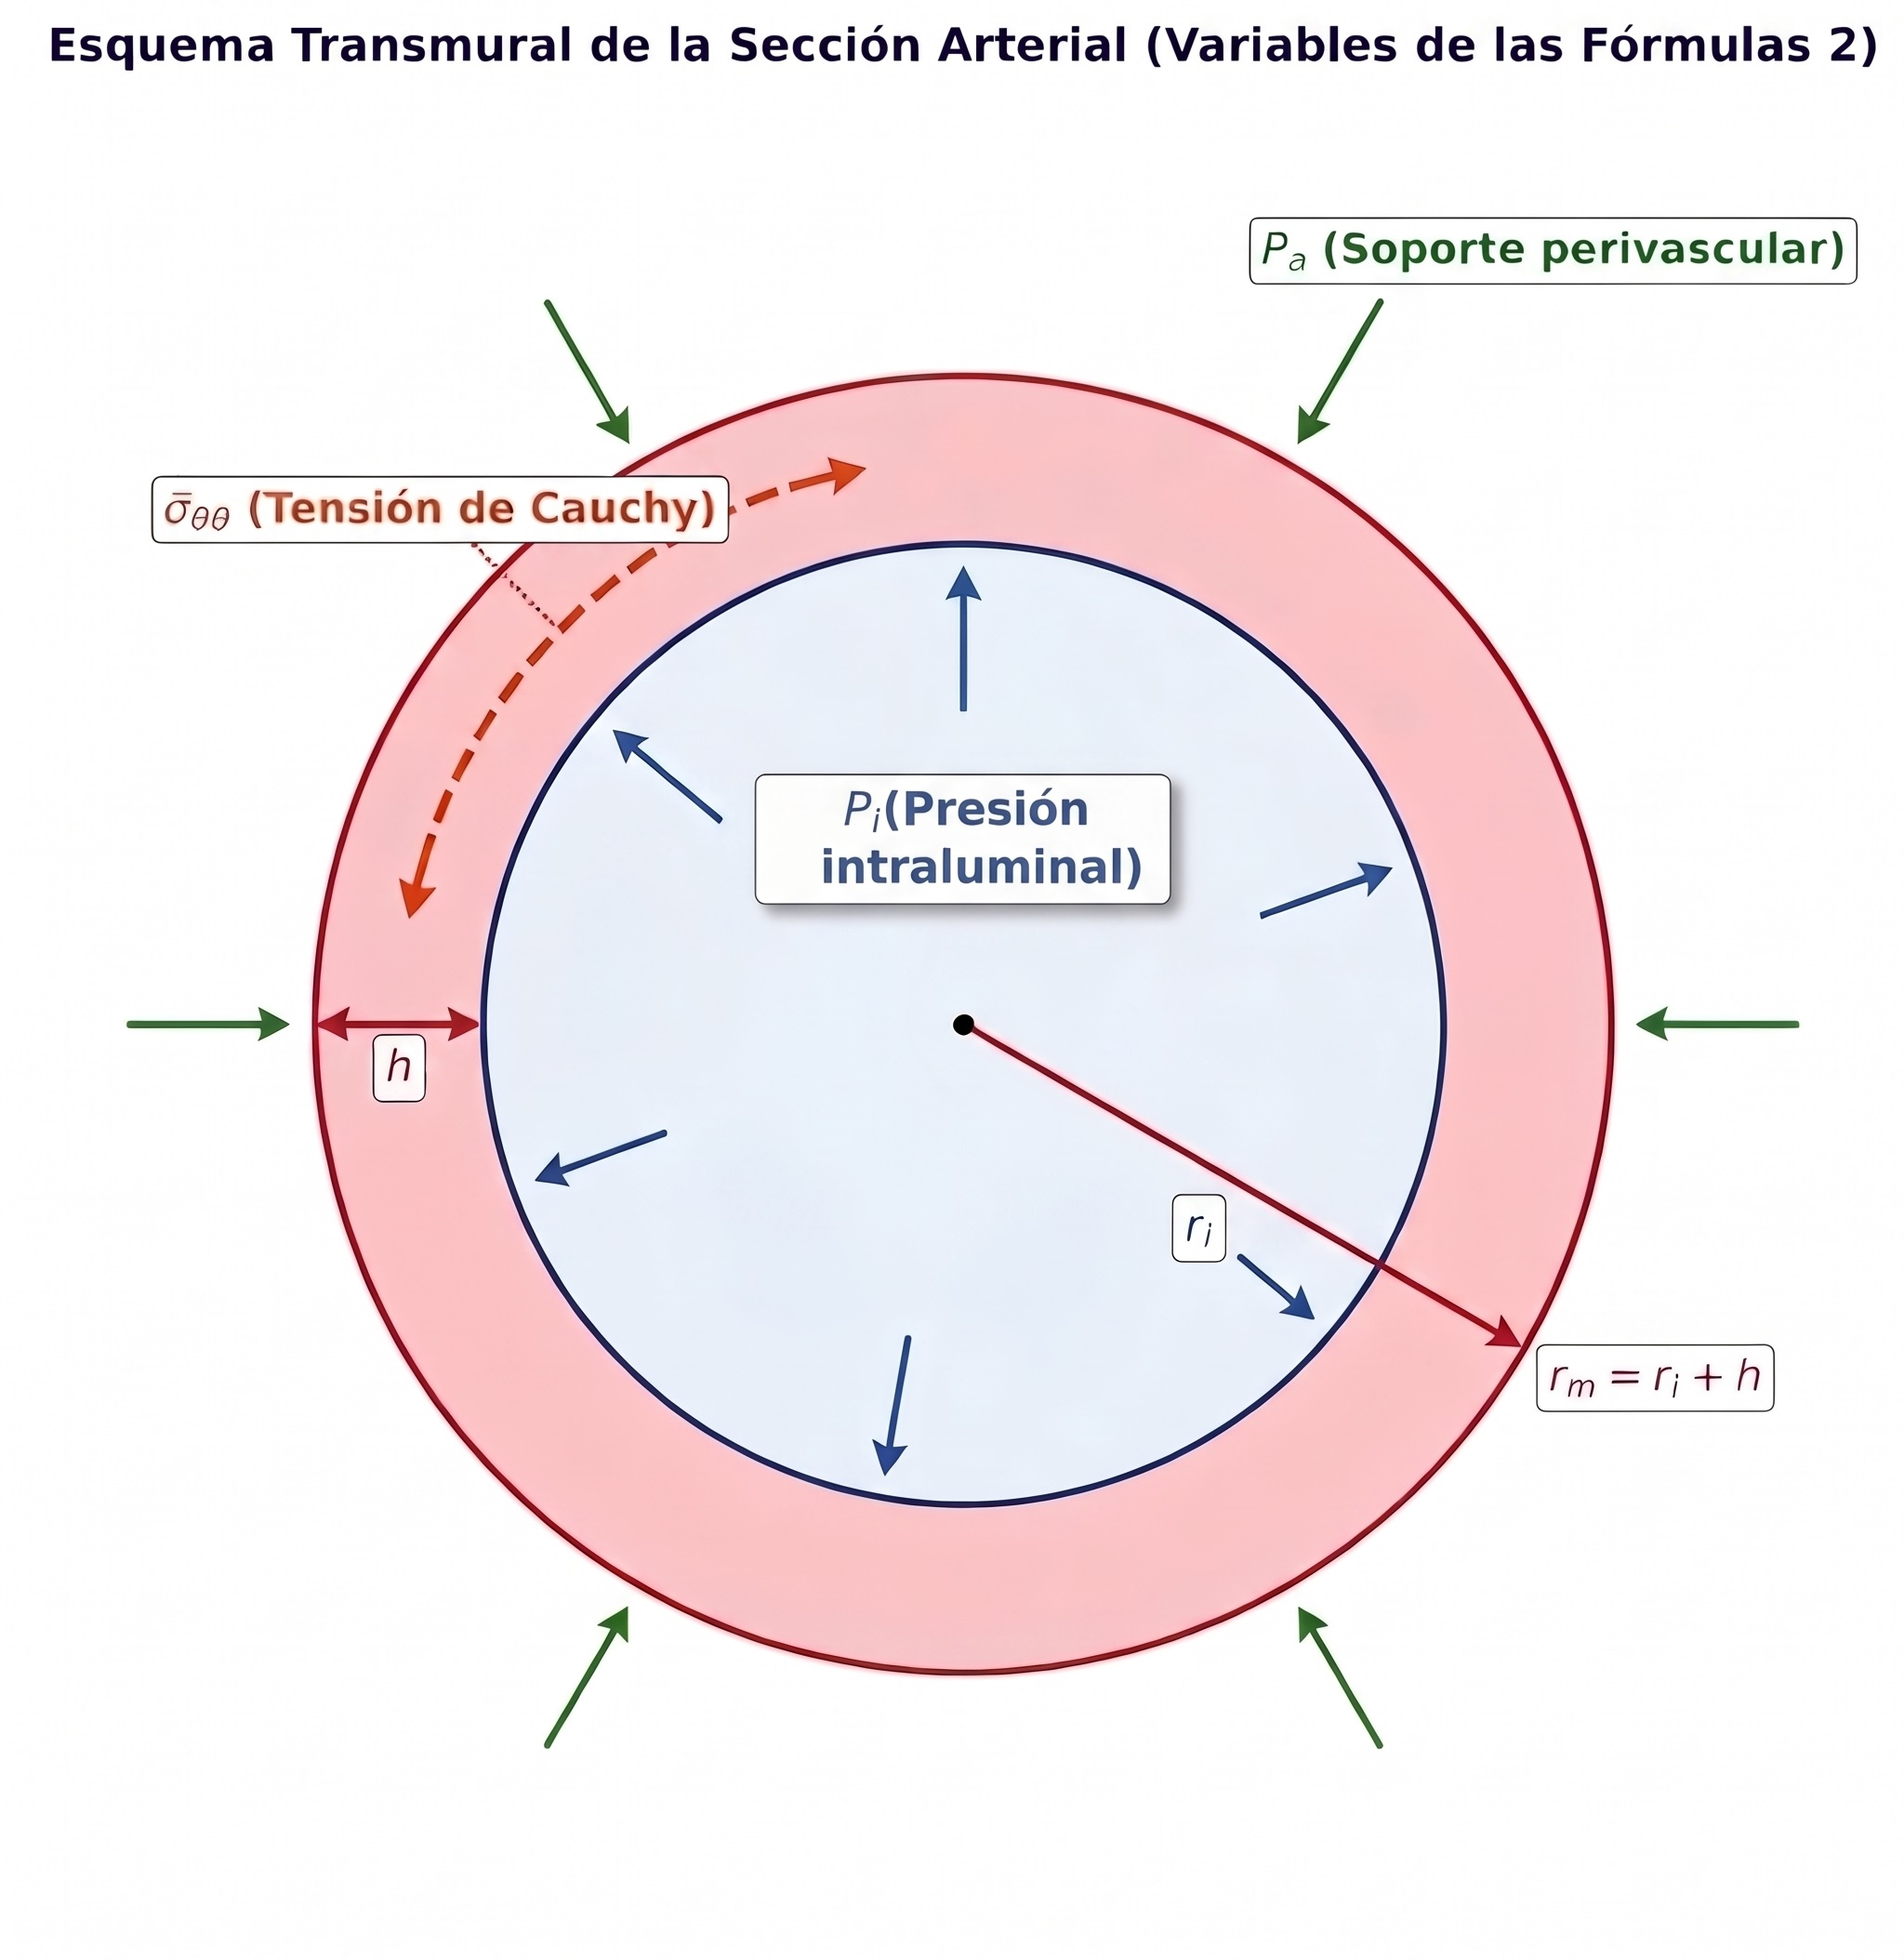
\includegraphics[width=0.40\linewidth]{Esquema_Arteria.jpg}
\caption{\textbf{Esquema Transmural de la Sección Arterial (Variables de las Fórmulas 2)}: Representación de la sección transversal indicando el radio interno $r_i$, el espesor deformado $h$, el radio externo de la media $r_m = r_i + h$, la tensión de Cauchy circunferencial $\bar{\sigma}_{\theta\theta}$, la presión intraluminal $P_i$ y la presión de soporte perivascular $P_a$.}
\label{fig:esquema_arteria_seccion}
\end{figure}

\subsection{2.4 Ecuación de Equilibrio Radial de Cauchy y Modelo Perivascular}
En dirección radial $r$, la ecuación de equilibrio estático $\frac{d\sigma_{rr}}{dr} + \frac{\sigma_{rr} - \sigma_{\theta\theta}}{r} = 0$, integrando con la presión sanguínea interna ($\sigma_{rr}(r_i) = -P_i(t)$) y la presión perivascular externa ($\sigma_{rr}(r_m) = -P_a(t)$), resulta en:
\begin{equation}
P_i(t) = P_{\text{pared}}(t) + P_a(t), \qquad P_{\text{pared}}(t) = \bar{\sigma}_{\theta\theta} \ln\left(1 + \frac{h}{r_i}\right), \qquad P_a(t) = a \cdot e^{b \cdot \frac{r_m(t)}{r_{md}}}
\end{equation}

\subsection{2.5 Demostración Analítica del Sesgo de Laplace (Pared Delgada)}
La hipótesis de Ley de Laplace ($p_{\text{delgada}} = \bar{\sigma}_{\theta\theta}(h/r_i)$), expandiendo $\ln(1+x)$ en serie de Taylor para $x = h/r_i < 1$, genera un sesgo positivo sistemático:
\begin{equation}
\frac{p_{\text{delgada}}}{p_{\text{exacta}}} = \frac{x}{\ln(1+x)} \approx 1 + \frac{1}{2} \left( \frac{h}{r_i} \right) \implies \text{Error (\%)} \approx \frac{1}{2} \left( \frac{h}{r_i} \right) \times 100\%
\end{equation}

\subsection{2.6 Formulación de Santiago Urquiza (Tesis Doctoral, Cap. 3)}
A partir de la Ecuación (3.13) de Urquiza (2012) ($(p - p_{\text{ext}}) R = \sigma h \implies p = \sigma (h/R)$):
\begin{enumerate}
\item \textbf{Evaluación en el Radio Interno ($R = r_i$)}:
\begin{equation}
p_{\text{Urq}, r_i} = \bar{\sigma}_{\theta\theta} \left( \frac{h}{r_i} \right) \qquad \text{(Coincide con Laplace, sobreestima entre $+6.7\%$ y $+9.2\%$)}
\end{equation}
\item \textbf{Evaluación en el Radio Medio Transmural ($R = r_m = r_i + \frac{h}{2}$)}:
\begin{equation}
p_{\text{Urq}, r_m} = \bar{\sigma}_{\theta\theta} \left( \frac{h}{r_i + \frac{h}{2}} \right) = \bar{\sigma}_{\theta\theta} \left( \frac{h/r_i}{1 + \frac{1}{2}\left(\frac{h}{r_i}\right)} \right)
\end{equation}
Esta expresión constituye la \textbf{aproximación de Padé [1/1]} de $\ln(1+x)$, reduciendo el error analítico con respecto a la solución exacta de pared gruesa a menos del $0.26\%$.
\end{enumerate}

\subsection{2.7 Deducción Analítica de las Funciones Explícitas $P_i(\lambda_\theta)$}

\subsubsection{2.7.1 Deducción de la Función Explícita $P_i(\lambda_\theta)$ para Pared Gruesa Exacta (In Vivo)}
Para expresar la presión intraluminal $P_i$ como una función matemática explícita e independiente del estiramiento circunferencial $\lambda_\theta$, se acopla la ecuación de equilibrio transmural con la ley cinemática de conservación de masa bajo incompresibilidad estricta ($J = \lambda_r \lambda_\theta \lambda_z = 1$).

Suponiendo deformación plana en dirección axial ($\lambda_z \approx 1$), el área de la sección transversal de la pared arterial permanece constante entre la configuración no deformada ($\lambda_\theta = 1.000$, con radio $R_i$ y espesor $H_0$) y la configuración deformada ($\lambda_\theta$, con radio $r_i$ y espesor $h$):
\begin{equation}
A_0 = \pi \left( (R_i + H_0)^2 - R_i^2 \right) = \pi R_i^2 \left[ \left(1 + \left(\frac{h}{r_i}\right)_0\right)^2 - 1 \right]
\end{equation}
\begin{equation}
A(\lambda_\theta) = \pi \left( (r_i + h)^2 - r_i^2 \right) = \pi r_i^2 \left[ \left(1 + \frac{h}{r_i}(\lambda_\theta)\right)^2 - 1 \right]
\end{equation}
Igualando $A(\lambda_\theta) = A_0$ y dividiendo por $\pi r_i^2$, considerando que por definición de estiramiento medio $\lambda_\theta = \frac{r_i}{R_i}$:
\begin{equation}
\left(1 + \frac{h}{r_i}(\lambda_\theta)\right)^2 - 1 = \frac{1}{\lambda_\theta^2} \left[ \left(1 + \left(\frac{h}{r_i}\right)_0\right)^2 - 1 \right]
\end{equation}
Despejando el cociente cinemático de aspecto deformado $u(\lambda_\theta) = 1 + \frac{h}{r_i}(\lambda_\theta)$:
\begin{equation}
u(\lambda_\theta) = 1 + \frac{h}{r_i}(\lambda_\theta) = \sqrt{1 + \frac{\left(1 + (h/r_i)_0\right)^2 - 1}{\lambda_\theta^2}}
\end{equation}
Sustituyendo $u(\lambda_\theta)$ en la solución exacta de Cauchy ($P_i = P_{\text{pared}} + P_a = \bar{\sigma}_{\theta\theta} \ln(u) + P_a$), se obtiene la \textbf{Ley Explícita de Presión Intraluminal de Pared Gruesa}:
\begin{equation}
P_{i,\text{exacta}}(\lambda_\theta) = \frac{1}{2} \bar{\sigma}_{\theta\theta}(\lambda_\theta) \cdot \ln\left( 1 + \frac{\left(1 + (h/r_i)_0\right)^2 - 1}{\lambda_\theta^2} \right) + P_a
\end{equation}
donde $(h/r_i)_0$ es la relación espesor/radio de referencia en el estado libre de carga ($\lambda_\theta = 1.000$) y $P_a$ es la precarga perivascular externa de confinamiento.

\subsubsection{2.7.2 Deducción de la Función Explícita $P_i(\lambda_\theta)$ para el Modelo de Santiago Urquiza}
A partir de la formulación simplificada de Urquiza (2012) evaluada en el radio medio transmural $r_m = r_i + \frac{h}{2}$:
\begin{equation}
P_{\text{Urq},\text{pared}}(\lambda_\theta) = \bar{\sigma}_{\theta\theta}(\lambda_\theta) \cdot \left( \frac{\frac{h}{r_i}(\lambda_\theta)}{1 + \frac{1}{2}\frac{h}{r_i}(\lambda_\theta)} \right)
\end{equation}
A partir de la relación cinemática incompresible obtenida en la Ec. (9), sustituimos la expresión de $\frac{h}{r_i}(\lambda_\theta) = \sqrt{1 + \frac{\left(1+(h/r_i)_0\right)^2-1}{\lambda_\theta^2}} - 1$:
\begin{equation}
P_{\text{Urq},\text{pared}}(\lambda_\theta) = \bar{\sigma}_{\theta\theta}(\lambda_\theta) \cdot \left( \frac{\sqrt{1 + \frac{\left(1+(h/r_i)_0\right)^2-1}{\lambda_\theta^2}} - 1}{1 + \frac{1}{2}\left(\sqrt{1 + \frac{\left(1+(h/r_i)_0\right)^2-1}{\lambda_\theta^2}} - 1\right)} \right)
\end{equation}
Multiplicando numerador y denominador por 2 y simplificando términos algebraicos:
\begin{equation}
P_{\text{Urq},\text{pared}}(\lambda_\theta) = \bar{\sigma}_{\theta\theta}(\lambda_\theta) \cdot \left( \frac{2\left(\sqrt{1 + \frac{\left(1+(h/r_i)_0\right)^2-1}{\lambda_\theta^2}} - 1\right)}{\sqrt{1 + \frac{\left(1+(h/r_i)_0\right)^2-1}{\lambda_\theta^2}} + 1} \right)
\end{equation}
Sumando la presión de confinamiento perivascular $P_a$, se obtiene la \textbf{Ley Explícita de Presión de Urquiza}:
\begin{equation}
P_{i,\text{Urq}}(\lambda_\theta) = \bar{\sigma}_{\theta\theta}(\lambda_\theta) \cdot \left[ \frac{2\left(\sqrt{1 + \frac{\left(1+(h/r_i)_0\right)^2-1}{\lambda_\theta^2}} - 1\right)}{\sqrt{1 + \frac{\left(1+(h/r_i)_0\right)^2-1}{\lambda_\theta^2}} + 1} \right] + P_a
\end{equation}
\textbf{Interpretación de Aproximación Padé [1/1]}: Definiendo la función cinemática $u(\lambda_\theta) = \sqrt{1 + \frac{\left(1+(h/r_i)_0\right)^2-1}{\lambda_\theta^2}}$, la solución exacta utiliza $\ln(u)$, mientras que la solución de Urquiza utiliza el cociente $\frac{2(u-1)}{u+1}$. Como la aproximación de Padé [1/1] de $\ln(u)$ en torno a $u = 1$ es precisamente $\frac{2(u-1)}{u+1}$, la Ley de Urquiza aproxima analíticamente la integral de pared gruesa con un error relativo menor al $0.26\%$.

\subsubsection{2.7.3 Comparación Analítica y Error Relativo de Padé [1/1] vs. Laplace}
En la siguiente figura y tabla se presenta la evaluación puntual de la función logarítmica exacta $\ln(u)$, la approximante Padé [1/1] de Urquiza $\frac{2(u-1)}{u+1}$ y la Ley de Laplace $u-1$:

\begin{figure}[H]
\centering
\includegraphics[width=0.82\linewidth]{pade_vs_ln_comparativa.png}
\caption{\textbf{Comparación Analítica y Error Relativo}: Superior: Evaluada la función exacta de pared gruesa $\ln(u)$, la approximante Padé [1/1] de Urquiza $\frac{2(u-1)}{u+1}$ y la Ley de Laplace $u-1$. Inferior: Error relativo porcentual con respecto a $\ln(u)$. El sombreado dorado destaca el rango fisiológico arterial ($h/r_i \in [0.10, 0.20]$).}
\label{fig:pade_vs_ln}
\end{figure}

\begin{table}[H]
\centering
\caption{\textbf{Evaluación Numérica Puntual de la Approximante Padé [1/1] de Urquiza vs. Laplace}. Se demuestra que el modelo de Urquiza mantiene el error por debajo del $0.28\%$ en todo el rango fisiológico de la carótida ($h/r_i \in [0.10, 0.20]$), mientras que la Ley de Laplace genera un sesgo positivo del $+4.92\%$ al $+9.70\%$.}
\label{tab:pade_vs_ln}
\resizebox{\linewidth}{!}{%
\begin{tabular}{ccccccc}
\toprule
$\mathbf{u = 1 + h/r_i}$ & $\mathbf{h/r_i}$ \textbf{[-]} & $\mathbf{\ln(u)}$ \textbf{(Exacta)} & \textbf{Padé [1/1] (Urquiza)} & \textbf{Err. Urquiza [\%]} & \textbf{Laplace ($u-1$)} & \textbf{Err. Laplace [\%]} \\
\midrule
1.00 & 0.00 & 0.00000 & 0.00000 & \textbf{+0.000\%} & 0.00000 & +0.00\% \\
1.05 & 0.05 & 0.04879 & 0.04878 & \textbf{-0.020\%} & 0.05000 & +2.48\% \\
1.10 & 0.10 & 0.09531 & 0.09524 & \textbf{-0.076\%} & 0.10000 & +4.92\% \\
1.12 & 0.12 & 0.11333 & 0.11321 & \textbf{-0.107\%} & 0.12000 & +5.89\% \\
1.15 & 0.15 & 0.13976 & 0.13953 & \textbf{-0.162\%} & 0.15000 & +7.33\% \\
1.18 & 0.18 & 0.16551 & 0.16514 & \textbf{-0.228\%} & 0.18000 & +8.75\% \\
1.20 & 0.20 & 0.18232 & 0.18182 & \textbf{-0.276\%} & 0.20000 & +9.70\% \\
1.25 & 0.25 & 0.22314 & 0.22222 & \textbf{-0.413\%} & 0.25000 & +12.04\% \\
\bottomrule
\end{tabular}%
}
\end{table}

\subsection{2.8 Relación Teórica entre las Tensiones Experimentales y el Modelo de Coorte ($\bar{\sigma}_{\theta\theta}$)}
Es fundamental establecer la distinción metodológica entre las curvas experimentales individuales obtenidas en los trabajos originales de Masson et al. (2011) y los valores discretos parametrizados en las Tablas 3 a 6 del presente informe:

\begin{enumerate}
\item \textbf{Naturaleza de los Datos Experimentales Originales}: Las trayectorias reportadas en las figuras de la literatura no corresponden a mediciones directas mediante ensayos destructivos de tracción, sino que representan una \textbf{reconstrucción indirecta no invasiva}. Mediante ecografía de alta resolución (\textit{ecotracking}), los autores miden dinámicamente la cinemática geométrica del radio interno $r_i(t)$ y del espesor $h(t)$ a lo largo del ciclo cardíaco, mientras que la presión intraluminal total $P_i(t)$ se registra mediante tonometría de aplanamiento. A partir de estos registros, se aplica un modelo inverso de mecánica de medios continuos para estimar el estado tensional de cada sujeto.
\item \textbf{Diferenciación de las Tensiones Circunferenciales ($\sigma_{\theta\theta}$ vs. $\bar{\sigma}_{\theta\theta}$)}:
\begin{itemize}
\item La tensión de Cauchy local $\sigma_{\theta\theta}(r)$ no es uniforme a través del espesor de la pared arterial, sino que varía radialmente desde el radio interno ($r_i$) hasta el externo ($r_m$) de acuerdo con el equilibrio estático radial.
\item Por otro lado, la tensión con barra $\bar{\sigma}_{\theta\theta}$ tabulada en las cohortes representa el \textbf{valor representativo o característico} de la íntima-media utilizado para parametrizar el modelo de pared gruesa.
\end{itemize}
\item \textbf{Formulación Matemática de Acoplamiento}: La relación cuantitativa que vincula la presión neta experimentada por la estructura tisular ($P_{\text{pared}} = P_i - P_a$) con la tensión representativa $\bar{\sigma}_{\theta\theta}$ y la cinemática de deformación se rige estrictamente por la ecuación exacta de equilibrio en cilindros de pared gruesa:
\begin{equation}
\bar{\sigma}_{\theta\theta}(\lambda_\theta) = \frac{P_i(\lambda_\theta) - P_a}{\ln\left(1 + \frac{h(\lambda_\theta)}{r_i(\lambda_\theta)}\right)}
\end{equation}
Donde el factor logarítmico cuantifica la corrección geométrica de espesor finito frente a la aproximación de pared delgada, y $P_a$ representa la presión de confinamiento perivascular externo.
\end{enumerate}

\subsubsection*{Aclaración Física}
\noindent Es fundamental destacar la distinción física entre la presión neta resistida por la estructura de la pared ($P_{\text{pared}}$) y la presión intraluminal total de la sangre ($P_i = P_{\text{pared}} + P_a$):
\begin{itemize}
\item Para una tensión de Cauchy medida en la Figura 5a de $\bar{\sigma}_{\theta\theta} \approx 60\text{ kPa}$, la pared de la íntima-media soporta únicamente $P_{\text{pared}} \approx 7.79\text{ kPa}$ ($58.4\text{ mmHg}$).
\item El tejido perivascular circundante ejerce una presión externa de confinamiento de $P_a \approx 5.63\text{ kPa}$ ($42.2\text{ mmHg}$).
\item La suma de ambas componentes equilibra la presión intraluminal sanguínea total de $P_i \approx 13.42\text{ kPa}$ ($100.7\text{ mmHg}$), la cual coincide con la presión fisiológica media \textit{in vivo}.
\end{itemize}

\section{3. Función Analítica de Ajuste Ex Vivo (Figura 6a)}
Para el complejo Media-Íntima de Carótida Común (\textit{Donante VI r}, Sommer \& Holzapfel 2012), el ajuste optimizado mediante mínimos cuadrados no lineales proporciona la siguiente función analítica explícita:
\begin{equation}
P_i(\lambda_\theta) = 0.1427 \cdot \left( e^{11.9103(\lambda_\theta - 1)} - 1 \right) \quad [\text{kPa}]
\end{equation}

\section{4. Tabla Cuantitativa Resumen de Resultados}

\begin{table}[H]
\centering
\caption{\textbf{Cuantificación Comparativa Resumen de Presiones Intraluminales y Variables de las Fórmulas (2)}: Pared Gruesa Exacta vs. Modelo de Urquiza y Laplace. Se integran las tensiones de Cauchy ($\bar{\sigma}_{\theta\theta}$) de Masson et al. (2011) [Fig. 5a y 7a] y Sommer \& Holzapfel (2012) [Fig. 6a].}
\label{tab:resultados_cuantitativos_resumen}
\resizebox{\linewidth}{!}{%
\begin{tabular}{lccccccccccc}
\toprule
\textbf{Cohorte / Estudio} & $\mathbf{\lambda_\theta}$ & $\mathbf{r_i\text{ [mm]}}$ & $\mathbf{h\text{ [mm]}}$ & $\mathbf{r_m\text{ [mm]}}$ & $\mathbf{r_{md}\text{ [mm]}}$ & $\mathbf{\bar{\sigma}_{\theta\theta}\text{ [kPa]}}$ & $\mathbf{P_{\text{pared}}\text{ [kPa] (mmHg)}}$ & $\mathbf{P_a\text{ [kPa]}}$ & $\mathbf{P_{\text{total}}\text{ [kPa] (mmHg)}}$ & $\mathbf{p_{\text{Urq},r_m}\text{ [kPa]}}$ & \textbf{Err$_{r_m}$} \\
\midrule
Masson Jóvenes (\textit{Mean Young}, Fig. 5a) & 1.115 & 3.48 & 0.48 & 3.95 & 3.82 & 60.0 & 7.79 (58.4) & 5.63 & 13.42 (100.7) & 7.78 & -0.14\% \\
Masson Mayores (\textit{Mean Old}, Fig. 5a) & 1.092 & 3.77 & 0.62 & 4.39 & 4.25 & 72.0 & 11.15 (83.7) & 5.61 & 16.76 (125.7) & 11.13 & -0.20\% \\
Masson Hipertensos (\textit{Mean HT}, Fig. 7a) & 1.075 & 3.87 & 0.73 & 4.60 & 4.45 & 82.0 & 14.42 (108.2) & 5.98 & 20.40 (153.0) & 14.38 & -0.26\% \\
Sommer Fig 6a Fit ($\lambda_\theta = 1.20$) & 1.200 & 3.72 & 0.30 & 4.02 & --- & 18.2 & 1.43 (10.8) & 0.00 & 1.43 (10.8) & 1.43 & -0.05\% \\
Sommer Fig 6a Fit ($\lambda_\theta = 1.30$) & 1.300 & 4.03 & 0.28 & 4.31 & --- & 75.4 & 5.12 (38.4) & 0.00 & 5.12 (38.4) & 5.12 & -0.04\% \\
Sommer Fig 6a Fit ($\lambda_\theta = 1.40$) & 1.400 & 4.34 & 0.26 & 4.60 & --- & 289.4 & 17.09 (128.2) & 0.00 & 17.09 (128.2) & 17.09 & -0.03\% \\
\bottomrule
\end{tabular}%
}
\end{table}

\section{5. Tablas Cuantitativas de Resultados por Cohorte In Vivo ($\lambda_\theta \in [1.000, 1.180]$)}
A continuación se presentan las tablas cuantitativas desglosadas punto a punto para cada una de las cohortes \textit{in vivo} de Masson et al. (2011), utilizando la presión de referencia normotensa $P_0 = 13.32\text{ kPa} \equiv 100.0\text{ mmHg}$.

\subsection{5.1 Cohorte Jóvenes Normotensos (Mean Young, 21--42a)}
Parámetros: $(h/r_i)_0 = 0.1703$, $P_a = 5.63\text{ kPa}$ ($42.2\text{ mmHg}$). Punto fisiológico medido a $\lambda_\theta = 1.115$ con $\bar{\sigma}_{\theta\theta} = 60.0\text{ kPa}$.

\begin{table}[htbp]
\centering
\caption{\textbf{Valores Cuantitativos para Jóvenes Normotensos (\textit{Mean Young}, Fig. 5a)}. Evaluada discreta desde $\lambda_\theta = 1.000$ hasta $\lambda_\theta = 1.180$.}
\label{tab:young_detallada}
\resizebox{\linewidth}{!}{%
\begin{tabular}{cccccccccc}
\toprule
$\mathbf{\lambda_\theta}$ \textbf{[-]} & $\mathbf{\bar{\sigma}_{\theta\theta}}$ \textbf{[kPa]} & $\mathbf{h/r_i}$ \textbf{[-]} & $\mathbf{P_{\text{pared}}}$ \textbf{[kPa]} & $\mathbf{P_a}$ \textbf{[kPa]} & $\mathbf{P_{i,\text{exacta}}}$ \textbf{[kPa]} & $\mathbf{P_{i,\text{exacta}}}$ \textbf{[mmHg]} & $\mathbf{P_i/P_0}$ \textbf{[-]} & $\mathbf{P_{i,\text{Urq}}}$ \textbf{[kPa]} & \textbf{Err Urq. [\%]} \\
\midrule
1.000 & 0.00 & 0.170 & 0.00 & 5.63 & 5.63 & 42.2 & 0.422 & 5.63 & +0.00\% \\
1.020 & 5.45 & 0.164 & 0.83 & 5.63 & 6.46 & 48.4 & 0.484 & 6.46 & -0.02\% \\
1.040 & 13.00 & 0.158 & 1.91 & 5.63 & 7.54 & 56.6 & 0.566 & 7.54 & -0.05\% \\
1.060 & 22.65 & 0.153 & 3.22 & 5.63 & 8.85 & 66.4 & 0.664 & 8.84 & -0.06\% \\
1.080 & 34.39 & 0.148 & 4.73 & 5.63 & 10.36 & 77.7 & 0.777 & 10.36 & -0.07\% \\
1.100 & 48.24 & 0.143 & 6.43 & 5.63 & 12.06 & 90.4 & 0.905 & 12.05 & -0.08\% \\
\rowcolor{highlightcol} 1.115 & 60.00 & 0.139 & 7.81 & 5.63 & 13.44 & 100.8 & 1.008 & 13.43 & -0.08\% \\
1.120 & 64.18 & 0.138 & 8.29 & 5.63 & 13.92 & 104.4 & 1.044 & 13.91 & -0.08\% \\
1.140 & 82.23 & 0.133 & 10.29 & 5.63 & 15.92 & 119.4 & 1.194 & 15.91 & -0.08\% \\
1.160 & 102.37 & 0.129 & 12.42 & 5.63 & 18.05 & 135.4 & 1.354 & 18.04 & -0.08\% \\
1.180 & 124.61 & 0.125 & 14.67 & 5.63 & 20.30 & 152.2 & 1.523 & 20.28 & -0.08\% \\
\bottomrule
\end{tabular}%
}
\end{table}

\subsection{5.2 Cohorte Mayores Normotensos (Mean Old, 53--64a)}
Parámetros: $(h/r_i)_0 = 0.2072$, $P_a = 5.61\text{ kPa}$ ($42.1\text{ mmHg}$). Punto fisiológico medido a $\lambda_\theta = 1.092$ con $\bar{\sigma}_{\theta\theta} = 72.0\text{ kPa}$.

\begin{table}[htbp]
\centering
\caption{\textbf{Valores Cuantitativos para Mayores Normotensos (\textit{Mean Old}, Fig. 5a)}. Evaluada discreta desde $\lambda_\theta = 1.000$ hasta $\lambda_\theta = 1.180$.}
\label{tab:old_detallada}
\resizebox{\linewidth}{!}{%
\begin{tabular}{cccccccccc}
\toprule
$\mathbf{\lambda_\theta}$ \textbf{[-]} & $\mathbf{\bar{\sigma}_{\theta\theta}}$ \textbf{[kPa]} & $\mathbf{h/r_i}$ \textbf{[-]} & $\mathbf{P_{\text{pared}}}$ \textbf{[kPa]} & $\mathbf{P_a}$ \textbf{[kPa]} & $\mathbf{P_{i,\text{exacta}}}$ \textbf{[kPa]} & $\mathbf{P_{i,\text{exacta}}}$ \textbf{[mmHg]} & $\mathbf{P_i/P_0}$ \textbf{[-]} & $\mathbf{P_{i,\text{Urq}}}$ \textbf{[kPa]} & \textbf{Err Urq. [\%]} \\
\midrule
1.000 & 0.00 & 0.207 & 0.00 & 5.61 & 5.61 & 42.1 & 0.421 & 5.61 & +0.00\% \\
1.020 & 7.32 & 0.200 & 1.33 & 5.61 & 6.94 & 52.1 & 0.521 & 6.94 & -0.05\% \\
1.040 & 19.26 & 0.193 & 3.40 & 5.61 & 9.01 & 67.6 & 0.676 & 9.00 & -0.10\% \\
1.060 & 35.84 & 0.186 & 6.12 & 5.61 & 11.73 & 88.0 & 0.880 & 11.71 & -0.13\% \\
1.080 & 57.05 & 0.180 & 9.44 & 5.61 & 15.05 & 112.9 & 1.129 & 15.02 & -0.14\% \\
\rowcolor{highlightcol} 1.092 & 72.00 & 0.176 & 11.69 & 5.61 & 17.30 & 129.7 & 1.297 & 17.27 & -0.15\% \\
1.100 & 82.89 & 0.174 & 13.29 & 5.61 & 18.90 & 141.7 & 1.417 & 18.87 & -0.15\% \\
1.120 & 113.36 & 0.168 & 17.62 & 5.61 & 23.23 & 174.2 & 1.742 & 23.19 & -0.15\% \\
1.140 & 148.47 & 0.163 & 22.38 & 5.61 & 27.99 & 210.0 & 2.100 & 27.95 & -0.15\% \\
1.160 & 188.20 & 0.158 & 27.53 & 5.61 & 33.14 & 248.6 & 2.486 & 33.09 & -0.15\% \\
1.180 & 232.57 & 0.153 & 33.03 & 5.61 & 38.64 & 289.8 & 2.898 & 38.58 & -0.14\% \\
\bottomrule
\end{tabular}%
}
\end{table}



\subsection{5.3 Cohorte Normotensos de Control (Mean NT, 39--64a)}
Parámetros: $(h/r_i)_0 = 0.1852$, $P_a = 5.62\text{ kPa}$ ($42.2\text{ mmHg}$). Punto fisiológico medido a $\lambda_\theta = 1.095$ con $\bar{\sigma}_{\theta\theta} = 65.0\text{ kPa}$.

\begin{table}[htbp]
\centering
\caption{\textbf{Valores Cuantitativos para Normotensos de Control (\textit{Mean NT}, Fig. 7a)}. Evaluada discreta desde $\lambda_\theta = 1.000$ hasta $\lambda_\theta = 1.180$.}
\label{tab:nt_detallada}
\resizebox{\linewidth}{!}{%
\begin{tabular}{cccccccccc}
\toprule
$\mathbf{\lambda_\theta}$ \textbf{[-]} & $\mathbf{\bar{\sigma}_{\theta\theta}}$ \textbf{[kPa]} & $\mathbf{h/r_i}$ \textbf{[-]} & $\mathbf{P_{\text{pared}}}$ \textbf{[kPa]} & $\mathbf{P_a}$ \textbf{[kPa]} & $\mathbf{P_{i,\text{exacta}}}$ \textbf{[kPa]} & $\mathbf{P_{i,\text{exacta}}}$ \textbf{[mmHg]} & $\mathbf{P_i/P_0}$ \textbf{[-]} & $\mathbf{P_{i,\text{Urq}}}$ \textbf{[kPa]} & \textbf{Err Urq. [\%]} \\
\midrule
1.000 & 0.00 & 0.185 & 0.00 & 5.62 & 5.62 & 42.2 & 0.422 & 5.62 & +0.00\% \\
1.020 & 6.67 & 0.179 & 1.10 & 5.62 & 6.72 & 50.4 & 0.504 & 6.71 & -0.04\% \\
1.040 & 17.08 & 0.172 & 2.71 & 5.62 & 8.33 & 62.5 & 0.625 & 8.33 & -0.07\% \\
1.060 & 31.23 & 0.166 & 4.80 & 5.62 & 10.42 & 78.2 & 0.782 & 10.41 & -0.09\% \\
1.080 & 49.13 & 0.161 & 7.32 & 5.62 & 12.94 & 97.0 & 0.970 & 12.92 & -0.10\% \\
\rowcolor{highlightcol} 1.095 & 65.00 & 0.157 & 9.45 & 5.62 & 15.07 & 113.0 & 1.130 & 15.06 & -0.11\% \\
1.100 & 70.76 & 0.155 & 10.21 & 5.62 & 15.83 & 118.7 & 1.187 & 15.81 & -0.11\% \\
1.120 & 96.13 & 0.150 & 13.44 & 5.62 & 19.06 & 143.0 & 1.430 & 19.04 & -0.11\% \\
1.140 & 125.25 & 0.145 & 16.98 & 5.62 & 22.60 & 169.5 & 1.695 & 22.57 & -0.11\% \\
1.160 & 158.10 & 0.141 & 20.79 & 5.62 & 26.41 & 198.1 & 1.981 & 26.38 & -0.11\% \\
1.180 & 194.70 & 0.136 & 24.84 & 5.62 & 30.46 & 228.5 & 2.285 & 30.42 & -0.11\% \\
\bottomrule
\end{tabular}%
}
\end{table}


\subsection{5.4 Cohorte Hipertensos Tratados (Mean HT, 44--69a)}
Parámetros: $(h/r_i)_0 = 0.2197$, $P_a = 5.98\text{ kPa}$ ($44.8\text{ mmHg}$). Punto fisiológico medido a $\lambda_\theta = 1.075$ con $\bar{\sigma}_{\theta\theta} = 82.0\text{ kPa}$.

\begin{table}[htbp]
\centering
\caption{\textbf{Valores Cuantitativos para Hipertensos Tratados (\textit{Mean HT}, Fig. 7a)}. Evaluada discreta desde $\lambda_\theta = 1.000$ hasta $\lambda_\theta = 1.180$.}
\label{tab:ht_detallada}
\resizebox{\linewidth}{!}{%
\begin{tabular}{cccccccccc}
\toprule
$\mathbf{\lambda_\theta}$ \textbf{[-]} & $\mathbf{\bar{\sigma}_{\theta\theta}}$ \textbf{[kPa]} & $\mathbf{h/r_i}$ \textbf{[-]} & $\mathbf{P_{\text{pared}}}$ \textbf{[kPa]} & $\mathbf{P_a}$ \textbf{[kPa]} & $\mathbf{P_{i,\text{exacta}}}$ \textbf{[kPa]} & $\mathbf{P_{i,\text{exacta}}}$ \textbf{[mmHg]} & $\mathbf{P_i/P_0}$ \textbf{[-]} & $\mathbf{P_{i,\text{Urq}}}$ \textbf{[kPa]} & \textbf{Err Urq. [\%]} \\
\midrule
1.000 & 0.00 & 0.220 & 0.00 & 5.98 & 5.98 & 44.9 & 0.449 & 5.98 & +0.00\% \\
1.020 & 10.23 & 0.212 & 1.97 & 5.98 & 7.95 & 59.6 & 0.596 & 7.94 & -0.08\% \\
1.040 & 28.92 & 0.205 & 5.38 & 5.98 & 11.36 & 85.2 & 0.852 & 11.35 & -0.14\% \\
1.060 & 56.08 & 0.198 & 10.11 & 5.98 & 16.09 & 120.7 & 1.207 & 16.06 & -0.17\% \\
\rowcolor{highlightcol} 1.075 & 82.00 & 0.192 & 14.43 & 5.98 & 20.41 & 153.1 & 1.531 & 20.38 & -0.18\% \\
1.080 & 91.70 & 0.191 & 16.02 & 5.98 & 22.00 & 165.0 & 1.650 & 21.96 & -0.18\% \\
1.100 & 135.78 & 0.184 & 22.99 & 5.98 & 28.97 & 217.3 & 2.173 & 28.91 & -0.19\% \\
1.120 & 188.32 & 0.178 & 30.92 & 5.98 & 36.90 & 276.8 & 2.768 & 36.83 & -0.19\% \\
1.140 & 249.32 & 0.173 & 39.72 & 5.98 & 45.70 & 342.8 & 3.428 & 45.62 & -0.18\% \\
1.160 & 318.79 & 0.167 & 49.29 & 5.98 & 55.27 & 414.6 & 4.146 & 55.18 & -0.18\% \\
1.180 & 396.72 & 0.162 & 59.56 & 5.98 & 65.54 & 491.6 & 4.916 & 65.43 & -0.17\% \\
\bottomrule
\end{tabular}%
}
\end{table}

\section{6. Superposición de las Funciones Calculadas y Escala Normalizada}

\subsection{6.1 Respuesta Normalizada a la Presión Fisiológica de Referencia ($P_i / P_0$)}
A continuación se presenta la curva normalizada referenciada a la presión intraluminal media de un normotenso joven ($P_0 = 13.32\text{ kPa} \equiv 100\text{ mmHg}$), expresando las presiones como fracciones $P_i / P_0$:

\begin{figure}[H]
\centering
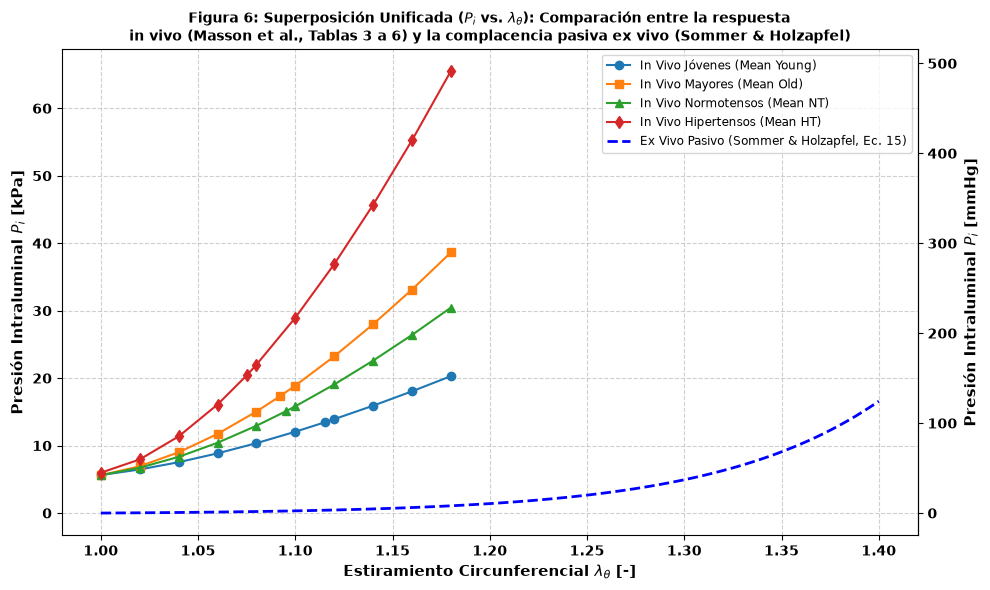
\includegraphics[width=0.72\linewidth]{superposicion_calculada.png}
\caption{\textbf{Superposición Unificada ($P_i$ vs. $\lambda_\theta$)}: Comparación entre la respuesta \textit{in vivo} confinada por tono muscular activo y soporte perivascular (Masson et al., Tablas 3 a 6) frente a la complacencia pasiva \textit{ex vivo} (Sommer \& Holzapfel, Figura 6a).}
\label{fig:superposicion_unificada}
\end{figure}\begin{figure}[H]
\centering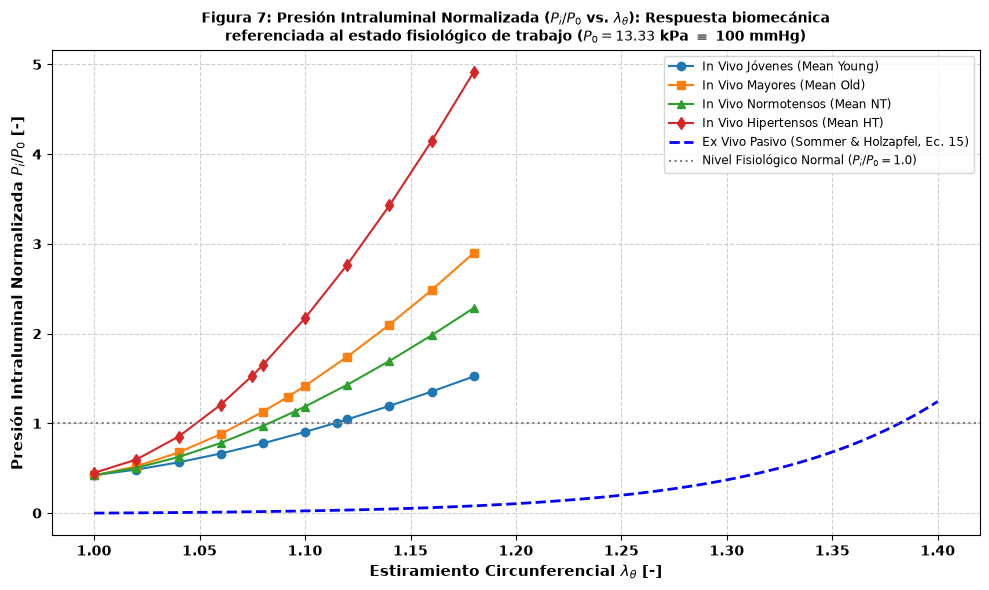
\includegraphics[width=0.72\linewidth]{superposicion_calculada_normalizada.png}
\caption{\textbf{Presión Intraluminal Normalizada ($P_i / P_0$ vs. $\lambda_\theta$)}: Respuesta biomecánica expresada como fracción de la presión fisiológica de trabajo ($P_0 = 13.32\text{ kPa} \equiv 100\text{ mmHg}$). La traza horizontal discontinua indica el nivel fisiológico normal $P/P_0 = 1.0$.}
\label{fig:superposicion_normalizada}
\end{figure}

\section{7. Conclusiones}
\begin{itemize}
\item \textbf{Efecto del Confinamiento Perivascular}: En arterias \textit{in vivo}, el soporte perivascular $P_a \approx 42\text{ mmHg}$ asume cerca del 40\% de la presión sanguínea total, permitiendo a la íntima-media operar a tensiones de Cauchy moderadas ($\bar{\sigma}_{\theta\theta} \approx 60\text{ kPa}$).
\item \textbf{Validación de la Formulación de Urquiza}: Evaluar la ecuación de Urquiza en el radio medio transmural ($r_m$) proporciona una precisión equivalente a la solución exacta de pared gruesa (error $< 0.26\%$), superando el sesgo positivo del $+6\%$ al $+9\%$ de Laplace ($r_i$).
\item \textbf{Respuesta Normalizada ($P/P_0$)}: Mientras la arteria \textit{in vivo} alcanza la presión normal ($P/P_0 = 1.0$) a un estiramiento de $\lambda_\theta = 1.115$, el tejido \textit{ex vivo} requiere estirarse hasta $\lambda_\theta = 1.383$ debido a la ausencia de tono muscular activo y confinamiento exterior.
\end{itemize}

\section{8. Bibliografía}
1. Masson, I., et al. (2011). A 3D constitutive model for human carotid arteries in vivo. \textit{Biomechanics and Modeling in Mechanobiology}, 10(4), 511--522.\\
2. Sommer, G., \& Holzapfel, G. A. (2012). 3D constitutive modeling of the biaxial mechanical response of human carotid arteries. \textit{Journal of the Mechanical Behavior of Biomedical Materials}, 5(1), 116--128.\\
3. Urquiza, S. A. (2012). Hemodinámica Computacional del Sistema Arterial Humano. Tesis Doctoral, Universidad Nacional de Cuyo / Instituto Balseiro.

\end{document}